\chapter{راهنمای استفاده از قالب \texttt{vruthesis}}

برای \gls{typeset} پایان‌نامه‌ها و رساله‌های دانشکده‌ی علوم ریاضی، می‌توان از قالب \texttt{vruthesis} استفاده نمود. در این فصل، ابتدا در بخش \ref{sec:file_org} به سازمان \glspl{file}ی مورد استفاده در این قالب پرداخته می‌شود. شیوه‌ی قرارگیری جدول‌ها، شکل‌ها، نمودارها، الگوریتم‌ها و قطعه‌برنامه‌ها در بخش \ref{sec:figs_tbls_algs_codes} ذکر می‌شود. بخش \ref{sec:eqs} به \gls{typeset}ِ روابط ریاضی اختصاص دارد. نکات مربوط به فرهنگ‌واژگان و نمادها در بخش \ref{sec:gloss} ذکر شده‌اند. در پایان، بخش \ref{sec:faq}، برخی از نکات سودمند در استفاده از این قالب را گوشزد می‌کند.

\section{سازمان \glspl*{file}ی قالب \texttt{vruthesis}}\label{sec:file_org} 
	متن یک پایان‌نامه به طور معمول، یک متن طولانی است. بنابراین، بهتر است تنظیمات \gls{formatting} و محتوای پایان‌نامه را از یکدیگر جدا کنیم. تنظیمات \gls{formatting} در \gls{file} \texttt{vruthesis.cls} آمده است. علاوه بر این، به منظور مدیریت بهتر بر محتوا، محتوای پایان‌نامه نیز بر اساس فصل در \glspl{file}ی متعدد، تقسیم‌بندی شده‌اند. به منظور سادگی بیشتر، نمونه‌ی یک پایان‌نامه‌ی کارشناسی ارشد و نمونه‌ی یک رساله‌ی دکتر در \gls{site} دانشکده قرار گرفته‌اند. هر یک از این نمونه‌ها، شامل چند \gls{file} مختلف هستند. فهرست این \glspl{file} و کاربرد هر یک از آن‌ها در جدول \ref{tbl:fileList} آمده است. استفاده از دستوراتی که در شرح آن‌ها، عبارت «در صورت وجود» آمده است؛ اختیاری است و در صورتی که این دستورات در \gls{file} \verb|data.tex| نیامده باشند یا به صورت توضیح درج شده باشند؛ خروجی به صورت متناسب تولید می‌گردد.

\begin{table}[ht]
	\caption[\glspl*{file}ی موجود در نمونه‌ی پایان‌نامه دانشکده.]{فهرست و کاربرد \glspl*{file}ی موجود در نمونه‌ی پایان‌نامه‌ی دانشکده‌ی علوم ریاضی.}
	\label{tbl:fileList}
	\centering
	\begin{tabular}{| R{0.60\textwidth} | L{0.25\textwidth} |}
		\hline 
		\textbf{شرح} & \textbf{نام \gls{file}} \\
		\hline
		\glspl{file} اصلی پایان‌نامه، شامل ارجاع به تنظیمات، محتوا و سایر دستورات & \texttt{thesis.tex} \\ \hline
		قالب \texttt{vruthesis} & \texttt{vruthesis.cls} \\ \hline
		اطلاعات مربوط به صفحات ابتدایی و انتهایی پایان‌نامه مانند عنوان (لاتین)، چکیده (لاتین) و مانند آن & \texttt{data.tex} \\ \hline
		تعریف منابع و مآخذ به صورت \texttt{bibtex} &  \texttt{references.bib} \\ \hline
		\gls{formatting} مراجع مطابق با استاندارد \lr{IEEE} با تغییرات مصوب گروه علوم‌کامپیوتر &  \texttt{ieeetr-fa-vru.bst} \\ \hline
		\gls{formatting} مراجع مطابق با استاندارد \lr{ACM} با در نظر گرفتن مراجع فارسی &  \texttt{acm-fa.bst} \\ \hline
		محتویات مربوط به فصل \lr{X} پایان‌نامه &  \texttt{chapterX.tex} \\ \hline
		محتویات مربوط به پیوست \lr{X} پایان‌نامه &  \texttt{appendixX.tex} \\ \hline
		اطلاعات مورد نیاز برای ساخت فهرست واژگان & \texttt{gloss.tex} \\ \hline
		فهرست اختصارات و نمادها & \texttt{acronym.tex} \\ \hline
	\end{tabular}
\end{table}

	برای تولید \gls{file} نهایی پایان‌نامه در قالب \gls{pdf}، لازم است تا از موتور \lr{TeX Live 2017} استفاده شود. دستورات مورد نیاز برای تولید خروجی، در شکل \ref{fig:output_cmd} ذکر شده‌اند. 
	
	\begin{figure}
		\begin{latin}
\centering
	\begin{verbatim}
	xelatex -synctex=-1 thesis.tex
bibtex8 -W -c cp1256fa thesis
xindy -L persian-variant1 -C utf8 -I xindy -M thesis.xdy 
        -t thesis.glg -o thesis.gls thesis.glo
xindy -L persian-variant1 -C utf8 -I xindy -M thesis.xdy 
        -t thesis.blg -o thesis.bls thesis.blo
xindy -L english -C utf8 -I xindy -M thesis.xdy -t thesis.alg 
        -o thesis.acr thesis.acn
xelatex -synctex=-1 thesis.tex
xelatex -synctex=-1 thesis.tex
	\end{verbatim}
	\end{latin}
\caption{دستورات لازم برای تولید خروجی نهایی به قالب \gls*{pdf}.}
\label{fig:output_cmd}
\end{figure}

در پایان‌نامه‌ی نمونه، $5$ فصل و یک پیوست درنظر گرفته شده است. در صورتی که در پایان‌نامه‌ی خود، به فصل‌های (پیوست‌های) بیشتری نیاز دارید؛ می‌توانید با تهیه‌ی یک رونوشت از \gls{file} \texttt{chapterX.tex} (\texttt{appendixX.tex}) و ذخیره‌ی آن به نام دلخواه، فصل (پیوست) جدیدی را ایجاد کنید. لازم به ذکر است که برای لحاظ شدن فصل جدید در خروجی، نیاز است تا در \gls{file} \texttt{thesis.tex}، دستور
\begin{latin}
	\begin{verbatim}
	\include{chapterX}
	\end{verbatim}
\end{latin}
را پس از {\verb|\chapter{نتیجه‌گیری}
در این فصل، نتیجه‌گیری پایان‌نامه‌ی خود را درج کنید.
			|} یا آخرین فصل اضافه شده، قرار دهید. به طور مشابه، برای لحاظ شدن پیوست جدید در خروجی، لازم است تا دستور \verb|\include{appendixX}| پس از \verb|\chapter{یک پیوست}
مطالب این پیوست بر اساس راهنمای نگارش پایان‌نامه‌های تحصیلات تکمیلی در \cite{vru_grad_rules} تهیه شده‌اند. 

	\begin{figure}
		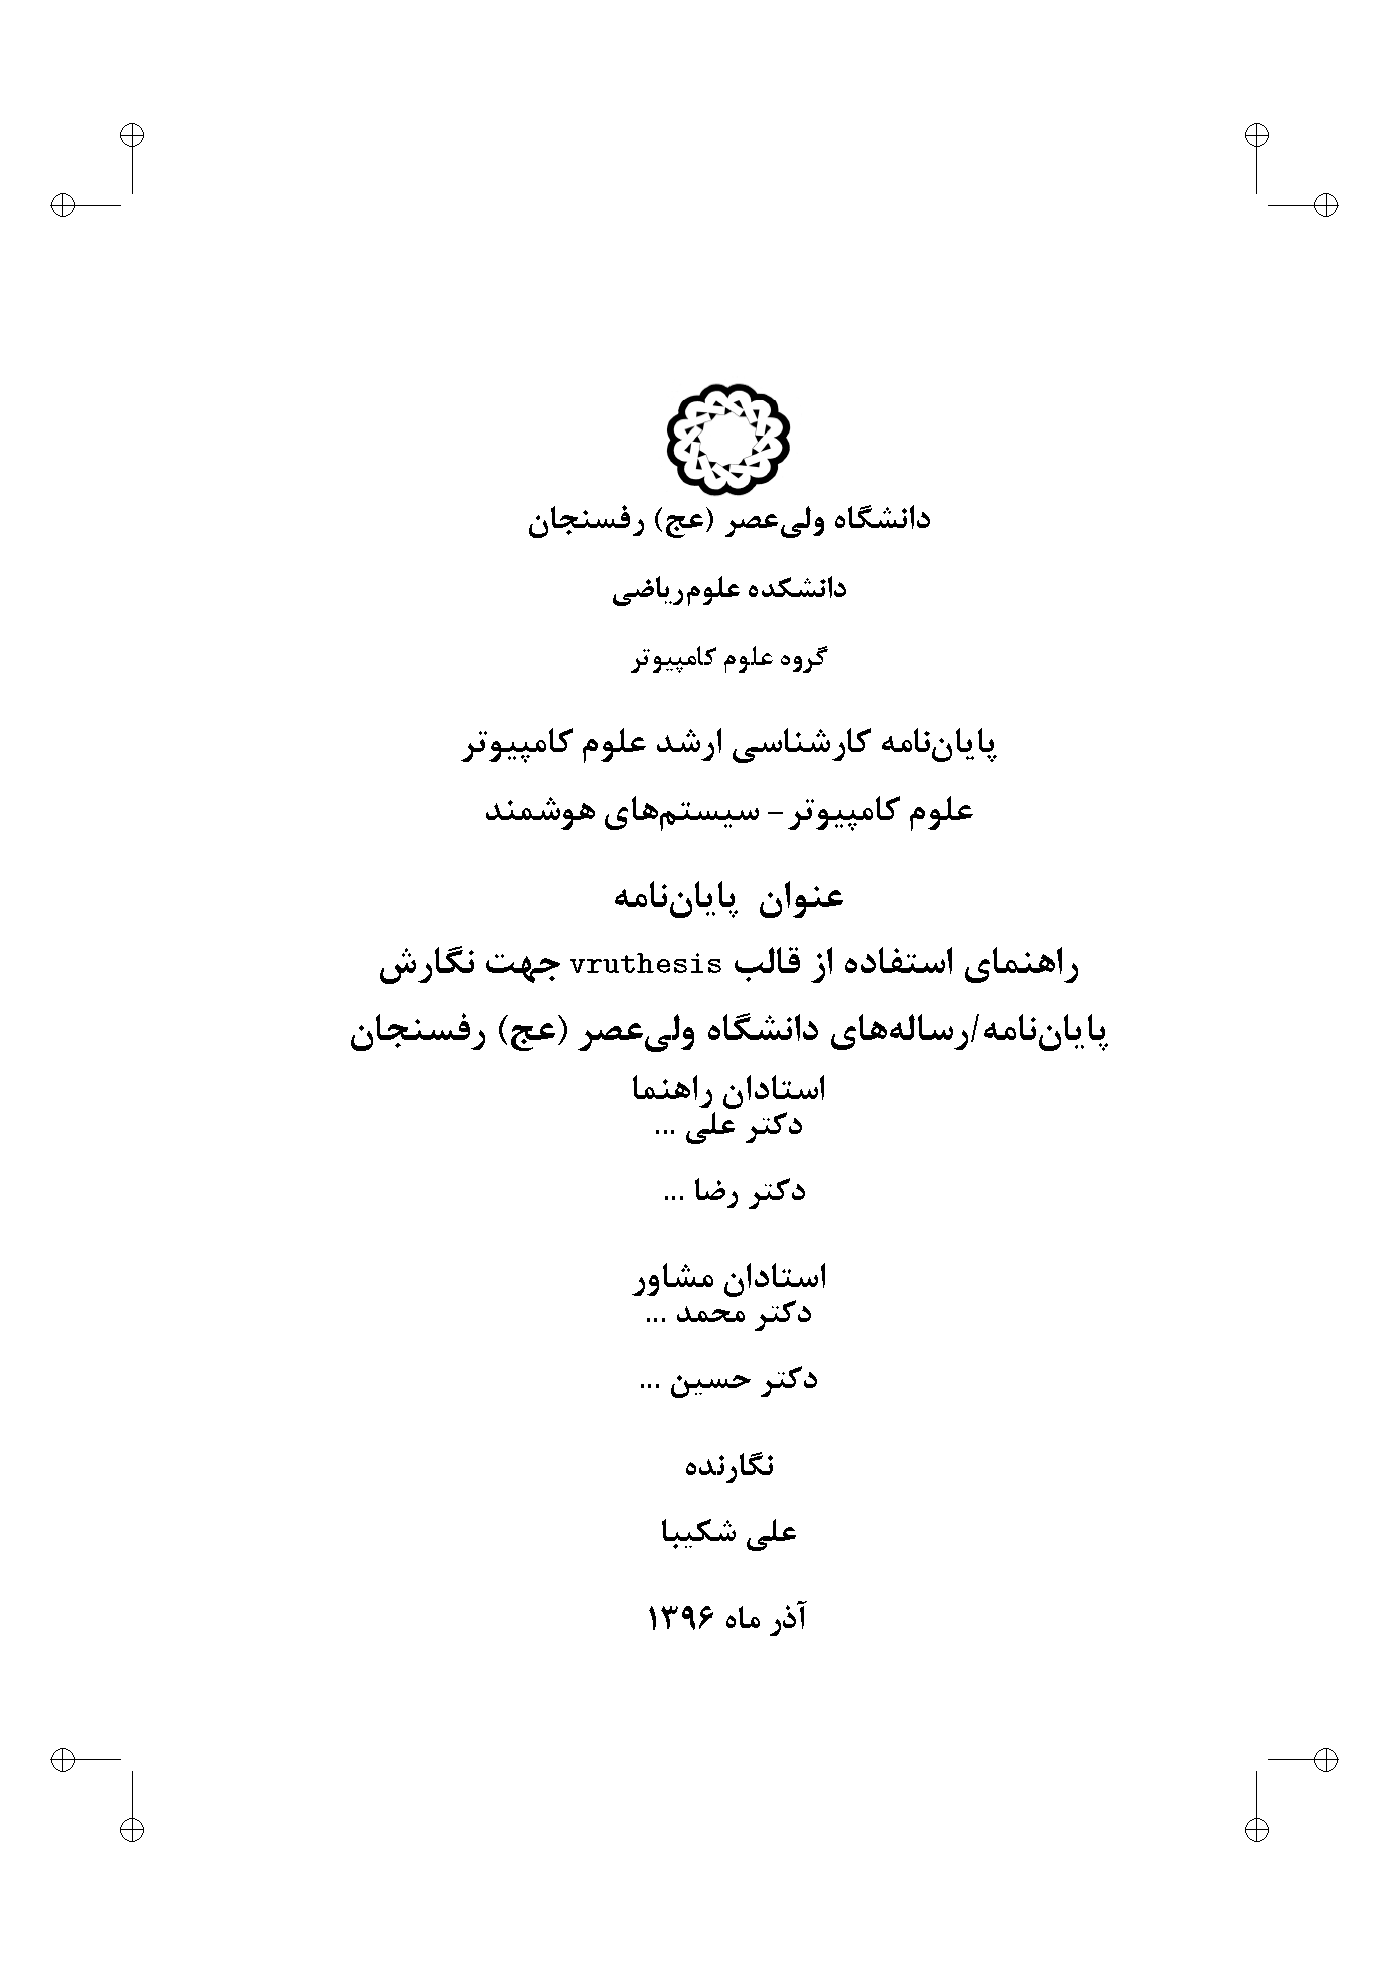
\includegraphics[width=\textwidth]{a.png}
		\caption{نمونه‌ی صفحه‌ی اول پایان‌نامه‌ی کارشناسی ارشد.}
		\label{app1}
	\end{figure}

	\begin{figure}
		
\includegraphics[width=\textwidth]{b.png}
		\caption{نمونه‌ی تصویب‌نامه‌ی پایان‌نامه‌ی کارشناسی ارشد.}
		\label{app2}
	\end{figure}

	\begin{figure}
		
\includegraphics[width=\textwidth]{d.png}
		\caption{تعهدات حقوقی.}
		\label{app4}
	\end{figure}

	\begin{figure}
		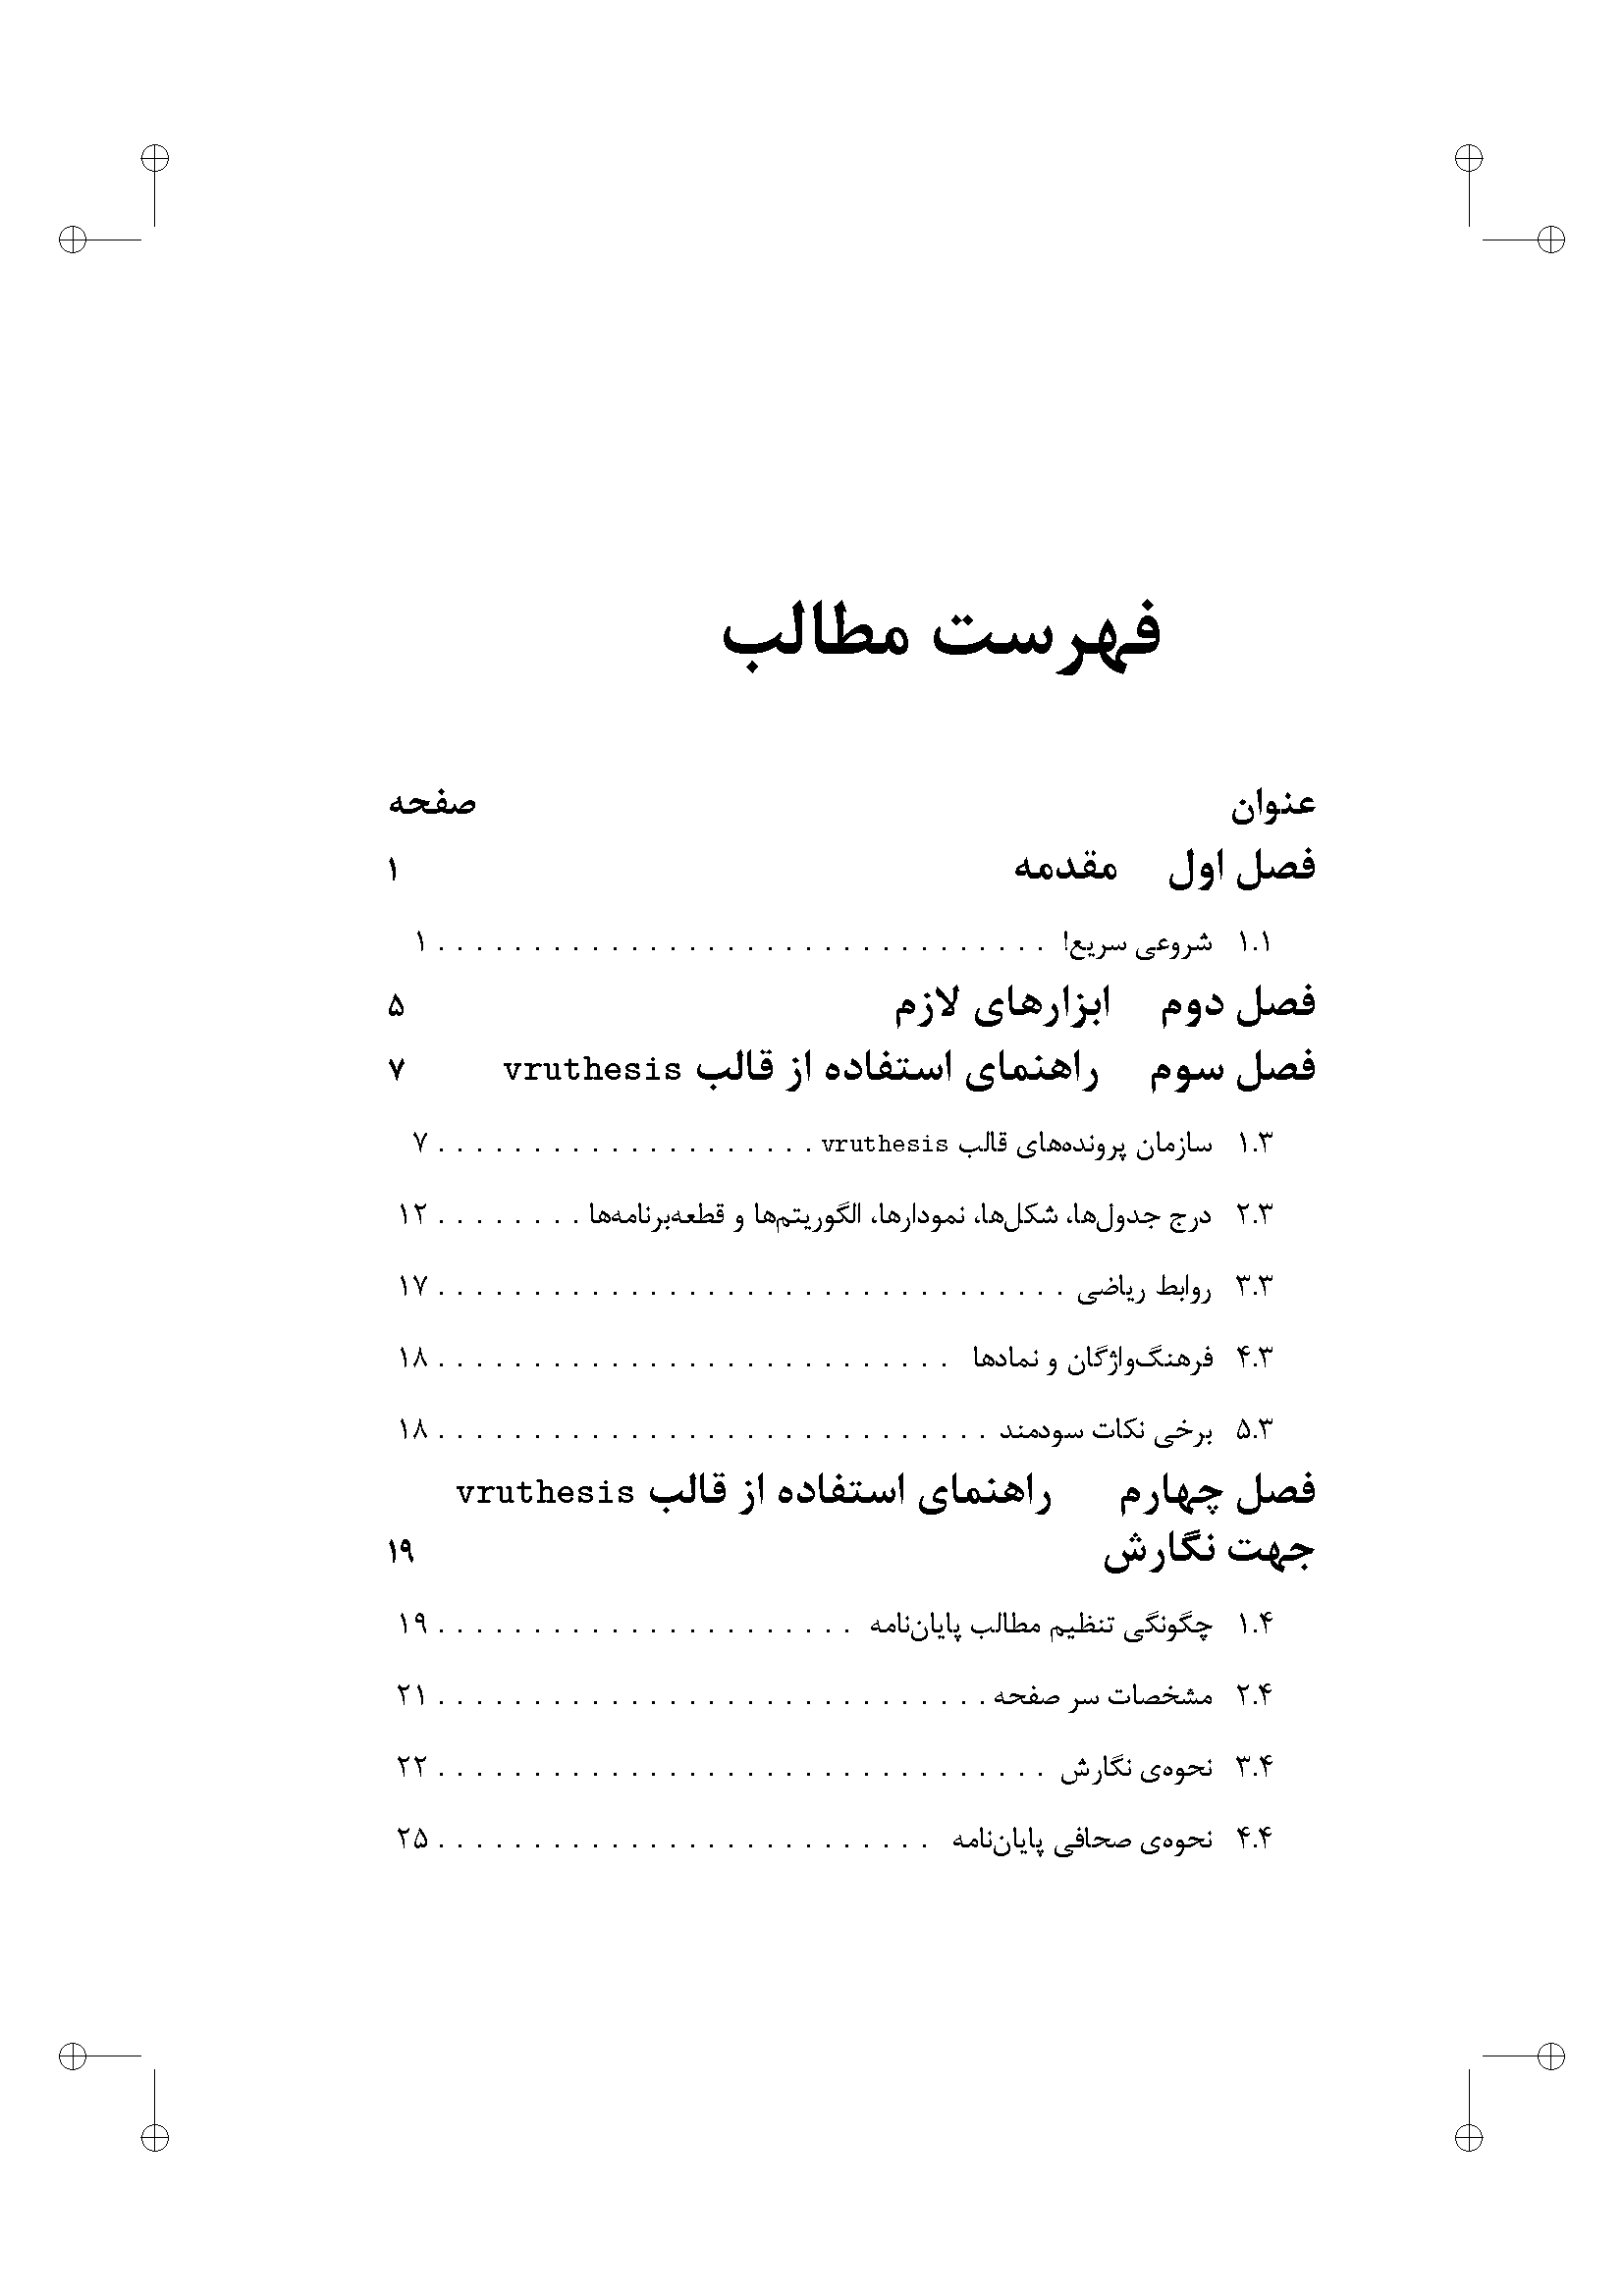
\includegraphics[width=\textwidth]{e.png}
		\caption{نمونه‌ای از فهرست مطالب.}
		\label{app5}
	\end{figure}

	\begin{figure}
		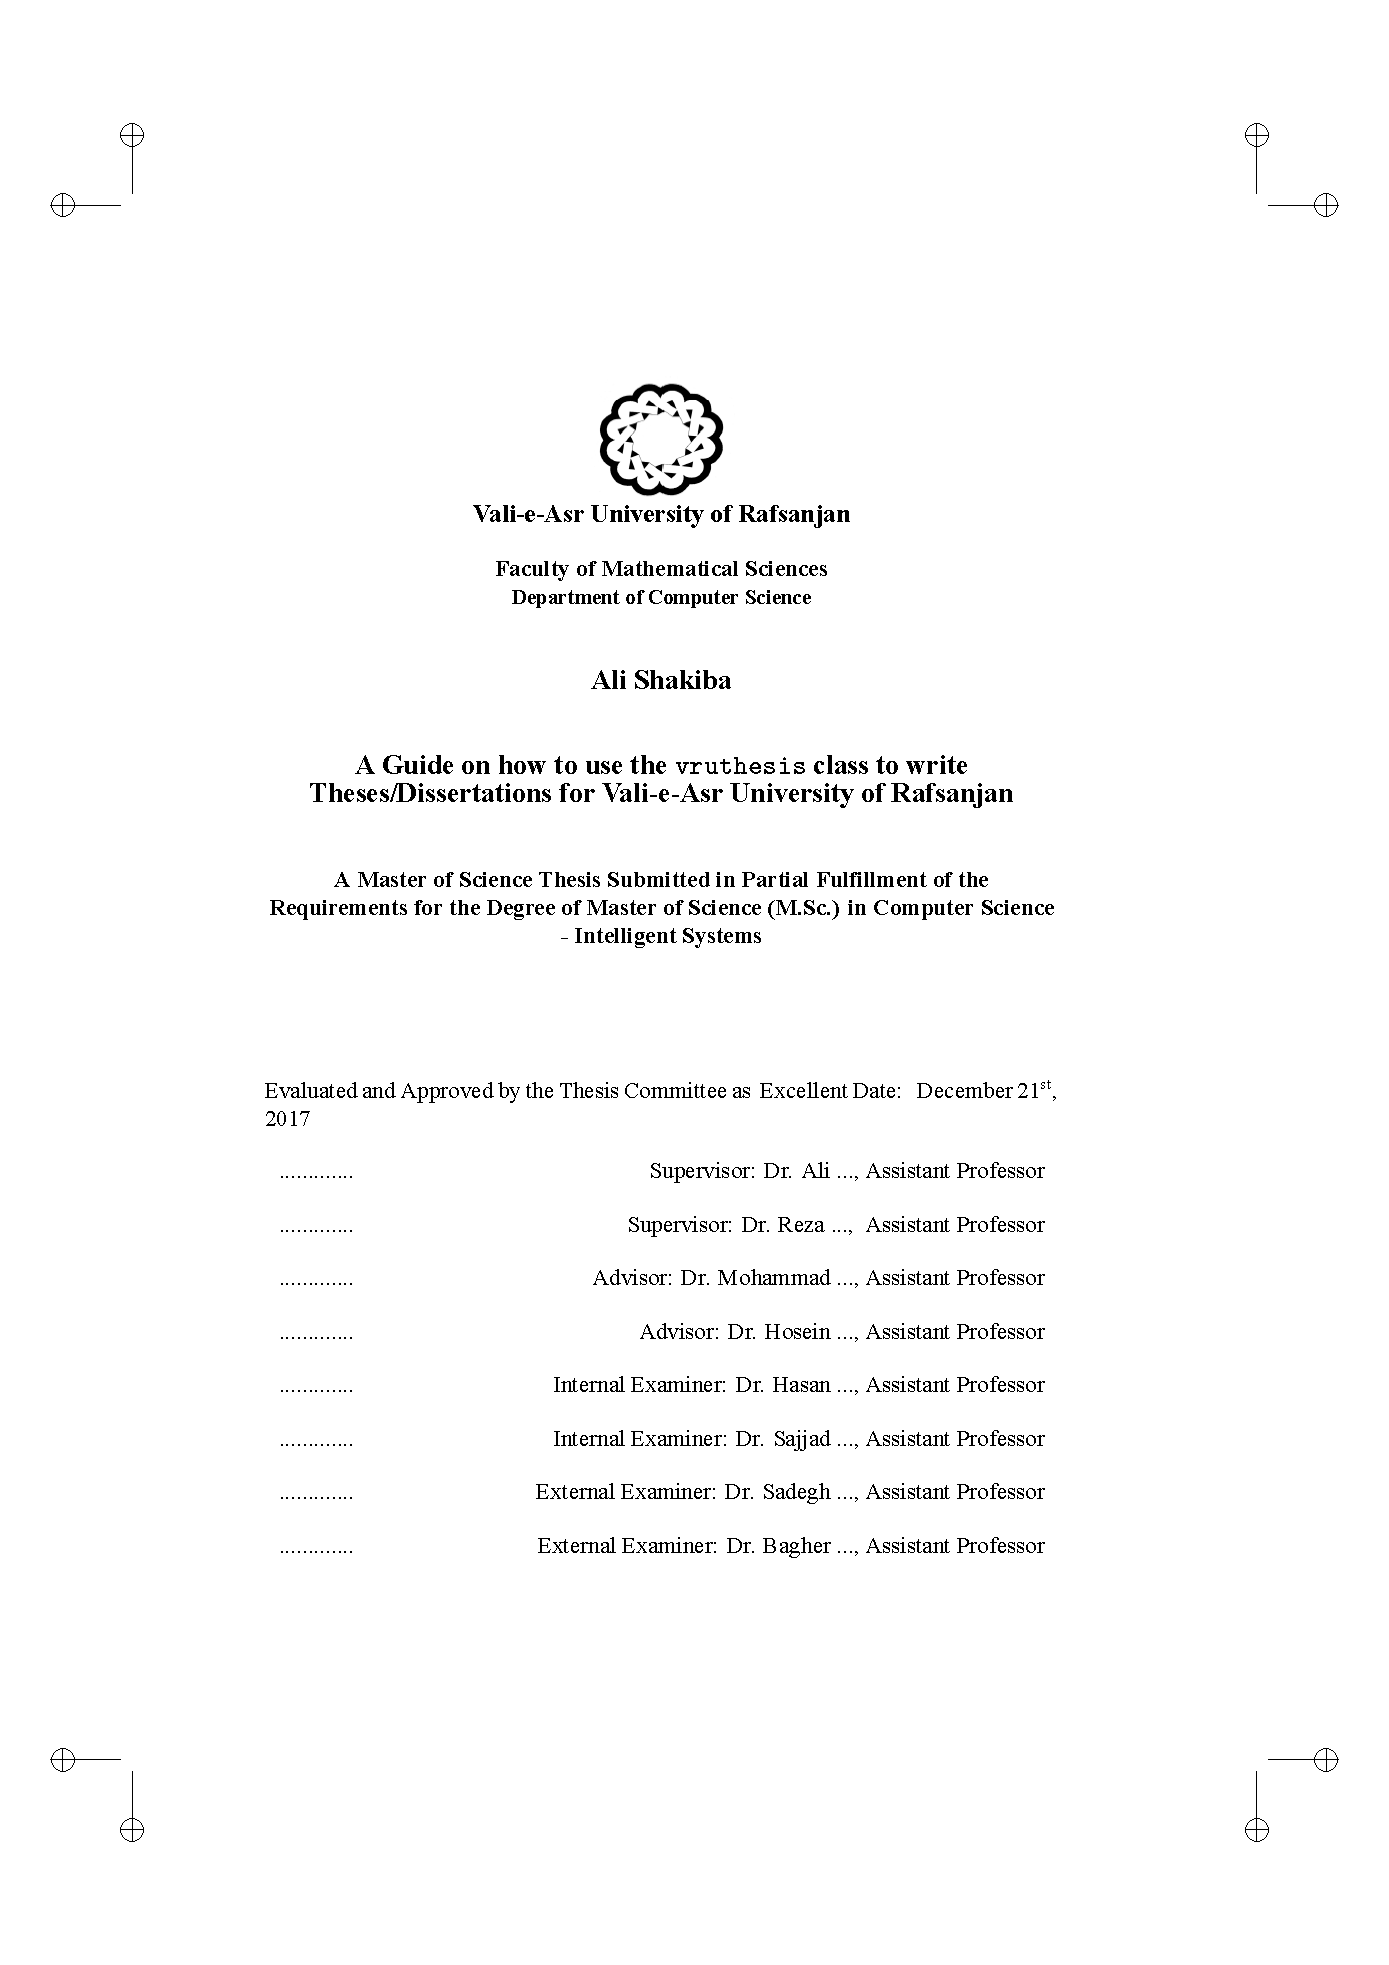
\includegraphics[width=\textwidth]{c.png}
		\caption{نمونه‌ی تصویب‌نامه‌ی پایان‌نامه‌ی کارشناسی ارشد به زبان انگلیسی.}
		\label{app3}
	\end{figure}

	\begin{figure}
		
\includegraphics[width=\textwidth]{f.png}
		\caption{نمونه‌ی صفحه‌ی آخر پایان‌نامه‌ی کارشناسی ارشد.}
		\label{app6}
	\end{figure}
| قرار گیرد. 

	جهت تولید صفحات عنوان، ارزیابی، سپاسگزاری، تقدیم‌به و چکیده به هر دو زبان فارسی و انگلیسی، لازم است تا محتوای \gls{file} \texttt{data.tex} را به صورت مناسب، تکمیل کنید. دستورات مورد استفاده در این \gls{file} و کاربرد آن‌ها در جدول \ref{tbl:data_cmds} آمده‌اند. این دستورات ممکن است در نگاه اوّل گیج‌کننده به نظر برسند. به همین دلیل، توصیه می‌شود که از \gls{file} \verb|data.tex| در پایان‌نامه‌ی نمونه استفاده کرده و تنها محتویات خود را در آن، جایگزین نمایید. 
	
	\begin{longtable}[c]{| L{.45\textwidth} | R{.45\textwidth} |}
		\caption{دستورات قابل استفاده در \gls*{file} \texttt{thesis.tex}.}
	\label{tbl:data_cmds}
	\\
	\hline	
		\textbf{شرح} & \textbf{دستور} \\ \hline
	\endfirsthead
	\multicolumn{2}{c}{ادامه‌ی جدول \ref{tbl:data_cmds}.} \\ \hline
	\textbf{شرح} & \textbf{دستور} \\ \hline
	\endhead
		\multicolumn{2}{c}{ادامه‌ی جدول در صفحه‌ی بعد.} \\
	\endfoot
		\hline
	\multicolumn{2}{c}{پایان جدول \ref{tbl:data_cmds}.} \\ 
	\endlastfoot
	
		عنوان دانشکده به فارسی &  \verb|\faculty{}| \\ \hline
		عنوان دانشکده به انگلیسی &  \verb|\facultyen{}| \\ \hline
		نام گروه به فارسی &  \verb|\department{}| \\ \hline
		نام گروه به انگلیسی &  \verb|\departmenten{}| \\ \hline
		عنوان رشته‌ی تحصیلی به فارسی &  \verb|\subject{}| \\ \hline
		عنوان رشته‌ی تحصیلی به انگلیسی &  \verb|\subjecten{}| \\ \hline
		عنوان گرایش تحصیلی به فارسی &  \verb|\field{}| \\ \hline
		عنوان گرایش تحصیلی به انگلیسی &  \verb|\fielden{}| \\ \hline
		عنوان پایان‌نامه به فارسی &  \verb|\title{}| \\ \hline
		عنوان پایان‌نامه به انگلیسی &  \verb|\titleen{}| \\ \hline
		نام و نام خانوادگی استاد راهنما به فارسی با پیشوند «دکتر» &  \verb|\firstsupervisor{}| \\ \hline
		نام و نام خانوادگی استاد راهنما به انگلیسی با پیشوند «\lr{Dr.}» &  \verb|\firstsupervisoren{}| \\ \hline
		رتبه‌ی علمی استاد راهنما به فارسی &  \verb|\firstsupervisorrank{}| \\ \hline
		رتبه‌ی علمی استاد راهنما به انگلیسی &  \verb|\firstsupervisorranken{}| \\ \hline
		نام و نام خانوادگی استاد راهنمای دوم، در صورت وجود، به فارسی با پیشوند «دکتر» &  \verb|\secondsupervisor{}| \\ \hline
		نام و نام خانوادگی استاد راهنمای دوم، در صورت وجود، به انگلیسی با پیشوند «\lr{Dr.}» &  \verb|\secondsupervisoren{}| \\ \hline
		رتبه‌ی علمی استاد راهنمای دوم، در صورت وجود، به فارسی &  \verb|\secondsupervisorrank{}| \\ \hline
		رتبه‌ی علمی استاد راهنمای دوم، در صورت وجود، به انگلیسی &  \verb|\secondsupervisorranken{}| \\ \hline
		نام و نام خانوادگی استاد مشاور، در صورت وجود، به فارسی با پیشوند «دکتر» &  \verb|\firstadvisor{}| \\ \hline
		نام و نام خانوادگی استاد مشاور، در صورت وجود، به انگلیسی با پیشوند «\lr{Dr.}» &  \verb|\firstadvisoren{}| \\ \hline
		رتبه‌ی علمی استاد مشاور، در صورت وجود، به فارسی &  \verb|\firstadvisorrank{}| \\ \hline
		رتبه‌ی علمی استاد مشاور، در صورت وجود، به انگلیسی &  \verb|\firstadvisorranken{}| \\ \hline
		نام و نام خانوادگی استاد مشاور دوم، در صورت وجود، به فارسی با پیشوند «دکتر» &  \verb|\secondadvisor{}| \\ \hline
		نام و نام خانوادگی استاد مشاور دوم، در صورت وجود، به انگلیسی با پیشوند «\lr{Dr.}» &  \verb|\secondadvisoren{}| \\ \hline
		رتبه‌ی علمی استاد مشاور دوم، در صورت وجود، به فارسی &  \verb|\secondadvisorrank{}| \\ \hline
		رتبه‌ی علمی استاد مشاور دوم، در صورت وجود، به انگلیسی &  \verb|\secondadvisorranken{}| \\ \hline
		نام و نام خانوادگی استاد داور داخلی اول به فارسی با پیشوند «دکتر» &  \verb|\firstinternalreferee{}| \\ \hline
		نام و نام خانوادگی استاد داور داخلی اول به انگلیسی با پیشوند «\lr{Dr.}» &  \verb|\firstinternalrefereeen{}| \\ \hline
		رتبه‌ی علمی استاد داور داخلی اول به فارسی &  \verb|\firstinternalrefereerank{}| \\ \hline
		رتبه‌ی علمی استاد داور داخلی اول به انگلیسی &  \verb|\firstinternalrefereeranken{}| \\ \hline
		نام و نام خانوادگی استاد داور داخلی دوم، در صورت وجود، به فارسی با پیشوند «دکتر» &  \verb|\secondinternalreferee{}| \\ \hline
		نام و نام خانوادگی استاد داور داخلی دوم، در صورت وجود، به انگلیسی با پیشوند «\lr{Dr.}» &  \verb|\secondinternalrefereeen{}| \\ \hline
		رتبه‌ی علمی استاد داور داخلی دوم، در صورت وجود، به فارسی &  \verb|\secondinternalrefereerank{}| \\ \hline
		رتبه‌ی علمی استاد داور داخلی دوم، در صورت وجود، به انگلیسی &  \verb|\secondinternalrefereeranken{}| \\ \hline
		نام و نام خانوادگی استاد داور خارجی اول به فارسی با پیشوند «دکتر» &  \verb|\firstexternalreferee{}| \\ \hline
		نام و نام خانوادگی استاد داور خارجی اول به انگلیسی با پیشوند «\lr{Dr.}» &  \verb|\firstexternalrefereeen{}| \\ \hline
		رتبه‌ی علمی استاد داور خارجی اول به فارسی &  \verb|\firstexternalrefereerank{}| \\ \hline
		رتبه‌ی علمی استاد داور خارجی اول به انگلیسی &  \verb|\firstexternalrefereeranken{}| \\ \hline
		نام و نام خانوادگی استاد داور خارجی دوم، در صورت وجود، به فارسی با پیشوند «دکتر» &  \verb|\secondexternalreferee{}| \\ \hline
		نام و نام خانوادگی استاد داور خارجی دوم، در صورت وجود، به انگلیسی با پیشوند «\lr{Dr.}» &  \verb|\secondexternalrefereeen{}| \\ \hline
		رتبه‌ی علمی استاد داور خارجی دوم، در صورت وجود، به فارسی &  \verb|\secondexternalrefereerank{}| \\ \hline
		رتبه‌ی علمی استاد داور خارجی دوم، در صورت وجود، به انگلیسی &  \verb|\secondexternalrefereeranken{}| \\ \hline
		نام و نام خانوادگی استاد ناظر به فارسی با پیشوند «دکتر» &  \verb|\viewer{}| \\ \hline
		نام و نام خانوادگی استاد ناظر به انگلیسی با پیشوند «\lr{Dr.}» &  \verb|\vieweren{}| \\ \hline
		رتبه‌ی علمی استاد ناظر به فارسی &  \verb|\viewerrank{}| \\ \hline
		رتبه‌ی علمی استاد ناظر به انگلیسی &  \verb|\viewerranken{}| \\ \hline
		نام دانشجو به فارسی &  \verb|\name{}| \\ \hline
		نام دانشجو به انگلیسی &  \verb|\nameen{}| \\ \hline
		نام خانوادگی دانشجو به فارسی &  \verb|\surname{}| \\ \hline
		نام خانوادگی دانشجو به انگلیسی &  \verb|\surnameen{}| \\ \hline
		ماه و سال جلسه‌ی دفاع به تقویم شمسی، مانند آذر $1396$ &  \verb|\thesisdate{}| \\ \hline
		ماه و سال جلسه‌ی دفاع به تقویم میلادی، مانند \lr{December 2017} &  \verb|\thesisdateen{}| \\ \hline
		تعداد واحد پایان‌نامه به فارسی، مانند $6$ &  \verb|\credit{}| \\ \hline
		تعداد واحد پایان‌نامه به انگلیسی، مانند \lr{$6$} &  \verb|\crediten{}| \\ \hline
		تاریخ جلسه‌ی دفاع به تقویم شمسی، مانند $۱۳۹۶/۰۹/۳۰$ &  \verb|\defensedate{}| \\ \hline
		تاریخ جلسه‌ی دفاع به تقویم میلادی، مانند \lr{December 21${}^{\text{st}}$, 2017}  &  \verb|\defensedateen{}| \\ \hline
		نمره‌ی پایان‌نامه با اعداد فارسی مانند، $19.75$ &  \verb|\grade{}| \\ \hline
		نمره‌ی پایان‌نامه با اعداد انگلیسی مانند، \lr{$19.75$} &  \verb|\gradeen{}| \\ \hline
		نمره‌ی پایان‌نامه به حروف به زبان فارسی &  \verb|\letgrade{}| \\ \hline
		نمره‌ی پایان‌نامه به حروف به زبان انگلیسی  &  \verb|\letgradeen{}| \\ \hline
		درجه‌ی دفاع به فارسی &  \verb|\degree{}| \\ \hline
		درجه‌ی دفاع به انگلیسی &  \verb|\degreeen{}| \\ \hline
		متن تقدیم‌به به زبان فارسی &  \verb|\totext{}| \\ \hline
		متن سپاسگزاری به فارسی &  \verb|\ack{}| \\ \hline
		متن چکیده به فارسی &  \verb|\abstractfa{}| \\ \hline
		متن چکیده به انگلیسی &  \verb|\abstracten{}| \\ \hline
	\end{longtable}

		\section{درج جدول‌ها، شکل‌ها، نمودارها، الگوریتم‌ها و قطعه‌برنامه‌ها}\label{sec:figs_tbls_algs_codes}
		پایان‌نامه‌ی شما ممکن است دارای جدول‌ها، شکل‌ها، نمودارها، الگوریتم‌ها و قطعه‌برنامه‌های مختلفی باشد. در این قالب، سه نوع محتوا درنظر گرفته شده است:
		\begin{itemize}
			\item جدول که تنها برای نمایش جدول‌ها استفاده می‌شود.
				\item الگوریتم که تنها برای نمایش الگوریتم‌ها استفاده می‌شود. 
			\item شکل که برای نمایش نمودارها،  قطعه‌برنامه‌ها، \glspl{flowchart} و سایر موارد بصری مورد استفاده قرار می‌گیرد.
		\end{itemize}
		
		در ادامه، نمونه‌ای از هر یک از موارد فوق آمده است. جدول \ref{tbl1}، یک جدول با تعداد ستون‌های زیاد است که لازم است تا در صفحه‌ای جداگانه درج شود. قطعه کد تولیدکننده‌ی این جدول در شکل \ref{fig:tbl1} آمده است. 
		
			شکل \ref{fig:clus1} نمونه‌ای از یک خوشه‌بندی برای یک دادگان نمونه است. همچنین، الگوریتم \ref{fig:alg} نیز نمونه‌ای از یک الگوریتم را نشان می‌دهد. از شکل‌ها می‌توان به منظور نمایش نمودارها نیز استفاده کرد؛ مانند \ref{fig:chart}. همچنین، شکل \ref{fig:tbl1}، بیانگر یک قطعه‌کد در \lr{\LaTeX} است. 
			
			\begin{figure}
				\centering
				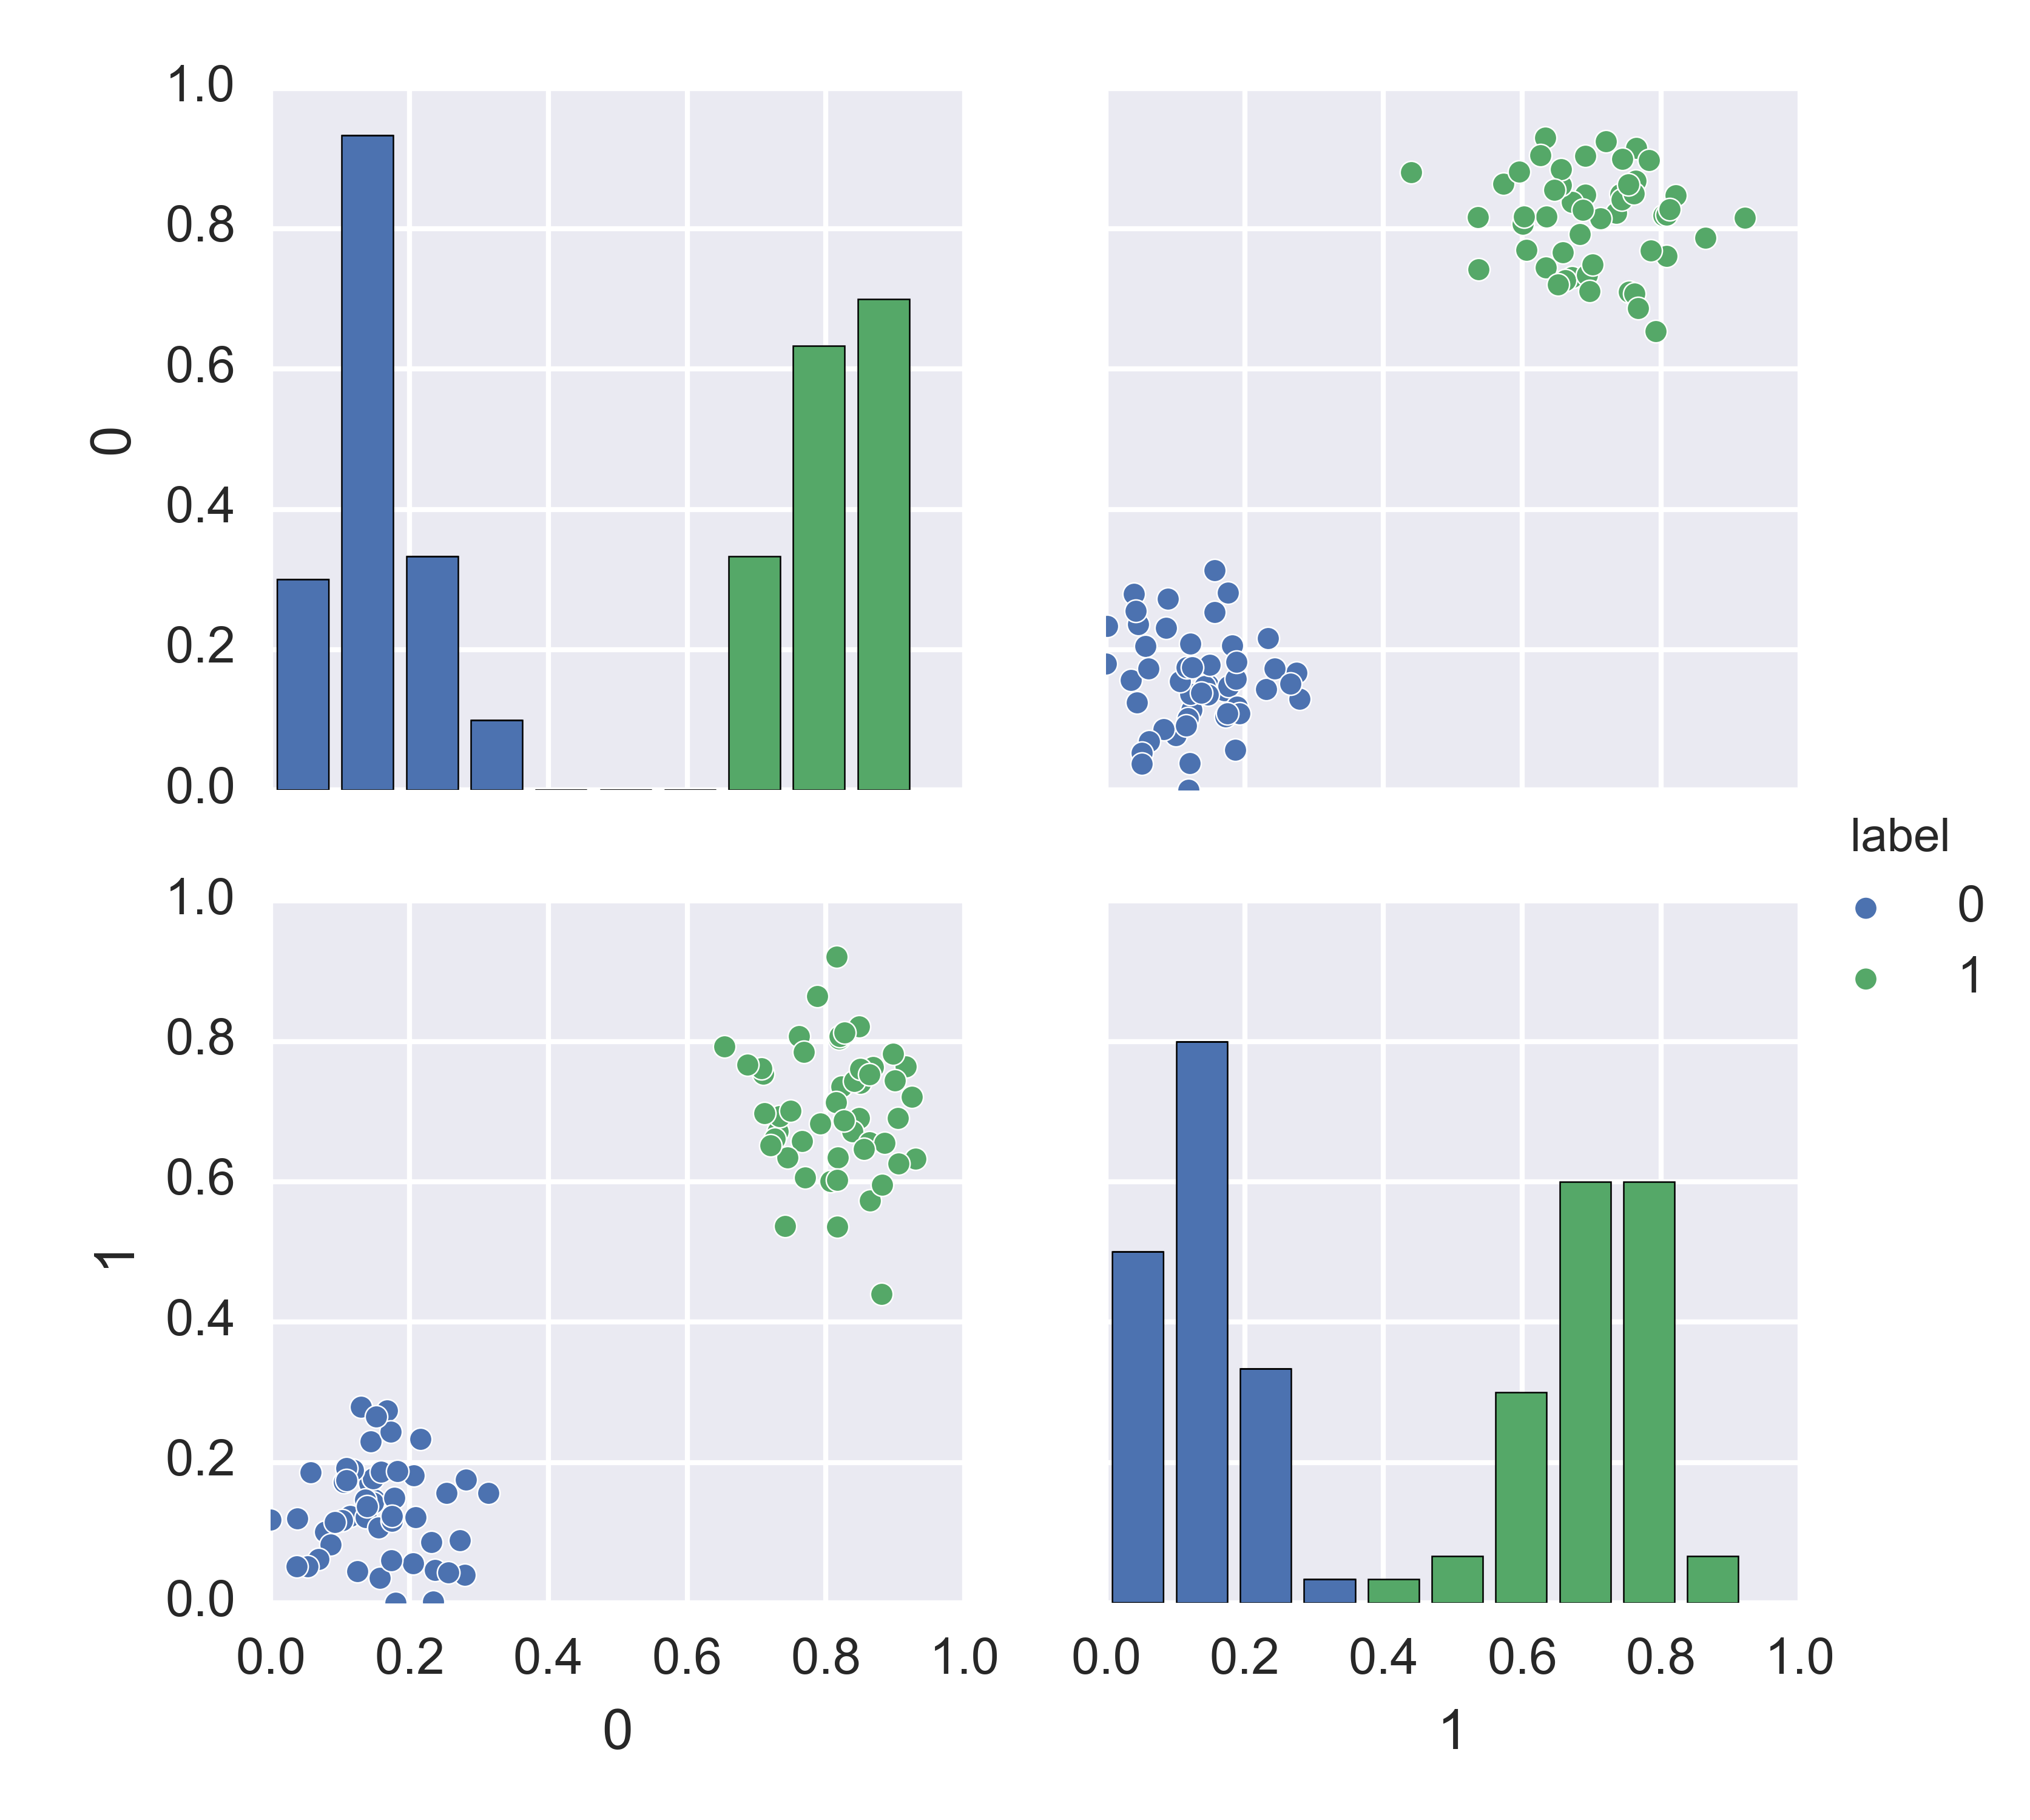
\includegraphics[width=.7\textwidth]{clus1}
				\caption{نمونه‌ای از یک خوشه‌بندی برای یک دادگان نمونه.}
				\label{fig:clus1}
			\end{figure}
		
		\begin{algorithm}
				\begin{latin}
		\begin{algorithmic}[1] % The number tells where the line numbering should start
        \Procedure{Euclid}{$a,b$} \Comment{\rl{ب.م.م. دو عدد صحیح مثبت $a$ و $b$}}
            \State $r\gets a \bmod b$
            \While{$r\not=0$} \Comment{\rl{اگر $r$ صفر باشد؛ پاسخ محاسبه شده است.}}
                \State $a \gets b$
                \State $b \gets r$
                \State $r \gets a \bmod b$
            \EndWhile\label{euclidendwhile}
            \State \textbf{return} $b$\Comment{\rl{ب.م.م. برابر با $b$ است.}}
        \EndProcedure
    \end{algorithmic}
    \end{latin}
    		\caption{الگوریتم اقلیدس برای محاسبه‌ی \gls*{gcd}.}
				\label{fig:alg}		
		\end{algorithm}	
			
			\begin{figure}
				\centering
				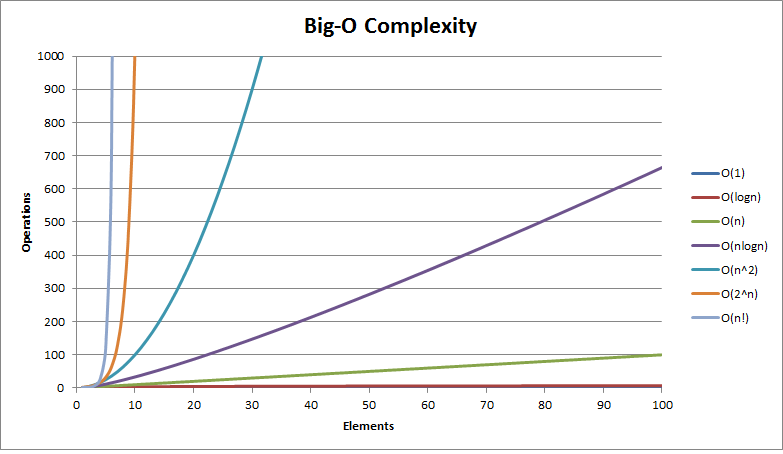
\includegraphics[width=.7\textwidth]{chart}
				\caption{نمونه‌ای از یک نمودار.}
				\label{fig:chart}
			\end{figure}
		
		\begin{figure}
			\centering
		\footnotesize
		\begin{myverbatim}
\begin{landscape}
  \begin{table}
    \caption{+rl[نمونه‌ای از یک جدول با تعداد ستون‌های زیاد.]}
    \label{tbl1}
    \centering
    \footnotesize
    \begin{tabular}{|r||c|c|c|c|c|c|c|c|c|c|c|c|c|c|c|}
      \hline
      \textbf{+rl[عنوان]} & $\alpha$ 
        & \multicolumn{5}{|c|}{$\gamma_1, \gamma_2, \ldots, \gamma_5$} 
        & $\beta$ & \multicolumn{8}{|c|}{+rl[سایر پارامترها]} \\ \hline
      +rl[نمونه‌ی اول]   &   74.85 &  0.32 &  13.99 &  91.25 &  80.74
         &  15.44 &  74.49 &  42.13 &
        1.08  &  32.98 &  18.74 &  46.83 &  81.28 &  31.52 &  8.29 \\
      +rl[نمونه‌ی دوم] &   22.76 &  48.61 &  
        70.77 &  22.77 &  3.81 &  45.05 &  
        70.55 &  33.20 &  1.40  &  24.42 &  79.06 &  
          30.38 &  24.95 &  19.77 &  44.59 \\
      +rl[نمونه‌ی سوم] &   55.67 &  36.98 &
          89.61 &  56.43 &  88.97 &  38.21 &  
        81.40 &  77.05 &  9.35 &  18.52 &  3.48 &  
          95.93 &  9.20 &  16.30 &  84.36 \\
      +rl[نمونه‌ی چهارم] &   60.31 &  88.25 &
          29.96 &  56.83 &  89.49 &  38.26 &  
        55.73 &  99.36 &  21.70 &  74.46 &  49.11 &  2.82
           &  25.47 &  2.90 &  84.58 \\
      +rl[نمونه‌ی پنجم] &   90.17 &  51.53 
        &  32.67 &  82.55 &  87.72 &  66.09 &  26.86 &  
        4.69 &  77.97 &  40.23 &  58.59 &  70.13 &  70.23 &
            80.73 &  64.88 \\
      +rl[نمونه‌ی ششم] &   74.92 
        &  52.33 &  98.68 &  63.75 &  30.10 &  7.32 &  91.70 &  
        72.76 &  42.50 &  26.72 &  23.33 &  73.55 & 
           77.37 &  32.79 &  15.60 \\
      +rl[نمونه‌ی هفتم] &   26.85 &  55.27
         &  5.12 &  88.21 &  4.92 &  70.78 &  
        75.26 &  32.03 &  25.11 &  61.81 &  44.24 &
            47.14 &  98.98 &  16.90 &  20.27 \\
      +rl[نمونه‌ی هشتم] &   84.33 &  12.53 &  36.00
         &  24.02 &  44.60 &  8.44 &  
        5.73 &  10.37 &  16.94 &  15.41 &  39.69 &
            43.74 &  10.43 &  73.96 &  26.51 \\
      +rl[نمونه‌ی نهم] &   59.21 &  47.46 & 
           97.27 &  87.05 &  84.65 &  17.95 &  50.05 &  
        38.68 &  20.09 &  46.99 &  12.47 &  10.92 & 
           78.38 &  74.53 &  31.83 \\
      +rl[نمونه‌ی دهم] &   97.61 &  33.47 &  67.78 
        &  69.95 &  60.95 &  88.40 &  
        59.64 &  18.22 &  57.49 &  97.76 &  40.31 &
            4.83 &  8.90 &  69.18 &  97.02 \\ \hline
    \end{tabular}
  \end{table}
\end{landscape}
		\end{myverbatim}
		\caption{قطعه‌کد مربوط به تولید جدول \ref{tbl1}.}
		\label{fig:tbl1}
		\end{figure}
	
	
		
		\begin{landscape}
			\begin{table}
				\caption{نمونه‌ای از یک جدول با تعداد ستون‌های زیاد.}
				\label{tbl1}
				\centering
				\footnotesize
				\begin{tabular}{|r||c|c|c|c|c|c|c|c|c|c|c|c|c|c|c|}
				\hline
				\textbf{عنوان} & $\alpha$ & \multicolumn{5}{|c|}{$\gamma_1, \gamma_2, \ldots, \gamma_5$} & $\beta$ & \multicolumn{8}{|c|}{سایر پارامترها} \\ \hline
نمونه‌ی اول 	&   74.85 &  0.32 &  13.99 &  91.25 &  80.74 &  15.44 &  74.49 &  42.13 &  1.08  &  32.98 &  18.74 &  46.83 &  81.28 &  31.52 &  8.29 \\
نمونه‌ی دوم &   22.76 &  48.61 &  70.77 &  22.77 &  3.81 &  45.05 &  70.55 &  33.20 &  1.40  &  24.42 &  79.06 &  30.38 &  24.95 &  19.77 &  44.59 \\
نمونه‌ی سوم &   55.67 &  36.98 &  89.61 &  56.43 &  88.97 &  38.21 &  81.40 &  77.05 &  9.35 &  18.52 &  3.48 &  95.93 &  9.20 &  16.30 &  84.36 \\
نمونه‌ی چهارم &   60.31 &  88.25 &  29.96 &  56.83 &  89.49 &  38.26 &  55.73 &  99.36 &  21.70 &  74.46 &  49.11 &  2.82 &  25.47 &  2.90 &  84.58 \\
نمونه‌ی پنجم &   90.17 &  51.53 &  32.67 &  82.55 &  87.72 &  66.09 &  26.86 &  4.69 &  77.97 &  40.23 &  58.59 &  70.13 &  70.23 &  80.73 &  64.88 \\
نمونه‌ی ششم &   74.92 &  52.33 &  98.68 &  63.75 &  30.10 &  7.32 &  91.70 &  72.76 &  42.50 &  26.72 &  23.33 &  73.55 &  77.37 &  32.79 &  15.60 \\
نمونه‌ی هفتم &   26.85 &  55.27 &  5.12 &  88.21 &  4.92 &  70.78 &  75.26 &  32.03 &  25.11 &  61.81 &  44.24 &  47.14 &  98.98 &  16.90 &  20.27 \\
نمونه‌ی هشتم &   84.33 &  12.53 &  36.00 &  24.02 &  44.60 &  8.44 &  5.73 &  10.37 &  16.94 &  15.41 &  39.69 &  43.74 &  10.43 &  73.96 &  26.51 \\
نمونه‌ی نهم &   59.21 &  47.46 &  97.27 &  87.05 &  84.65 &  17.95 &  50.05 &  38.68 &  20.09 &  46.99 &  12.47 &  10.92 &  78.38 &  74.53 &  31.83 \\
نمونه‌ی دهم &   97.61 &  33.47 &  67.78 &  69.95 &  60.95 &  88.40 &  59.64 &  18.22 &  57.49 &  97.76 &  40.31 &  4.83 &  8.90 &  69.18 &  97.02 \\ \hline
				\end{tabular}
			\end{table}
		\end{landscape}
	
		\section{روابط ریاضی}\label{sec:eqs}
		به طور معمول، بخش زیادی از یک پایان‌نامه در دانشکده‌ی علوم ریاضی، از روابط ریاضی تشکیل شده است. یک رابطه‌ی ریاضی را می‌توان به صورت \gls{inline} مانند $\int_{-\infty}^{+\infty} \sin x \mathrm{d} x$ نوشت. همچنین، می‌توان یک رابطه‌ی ریاضی را بدون شماره‌گذاری مانند
		$$
			A \wedge \left( B \vee C \right) = \left(A \wedge B \right) \vee \left( A \wedge C \right),
		$$
		نوشت. امّا، با توجه به زیادبودن تعداد روابط ریاضی، بهتر است در صورتی که به یک رابطه ارجاع داده می‌شود؛ آن را شماره‌گذاری نمایید؛ مانند
		\begin{equation}
			P \left(B_i \vert A \right) = \frac{P\left(A \vert B_i \right) P\left(B_i\right)}{\sum_j P\left(A \vert B_j \right) P\left(B_j\right)},
			\label{eq:1}
		\end{equation}
		که $i=1,\ldots,k$ است. بنابراین، می‌توان به سادگی به رابطه‌ی \ref{eq:1}، ارجاع داد. 
		
		همچنین، محیط‌های متنوعی برای \gls{typeset} قضیه‌ها، لم‌ها، گزاره‌ها، نتیجه‌ها، تعریف‌ها و مانند آن‌ها در نظر گرفته شده‌اند که در ادامه، نمونه‌های مختلفی از آن‌ها را مشاهده می‌کنید.
		
		\begin{theorem}[\cite{gary}]
			\label{}
			زبان $\mathrm{SAT} = \left\{ \left\langle \Phi \right\rangle \ \vert \ \text{\rl{ صدق‌پذیر است} } \Phi  \right\}$، مفروض است. داریم
			\begin{equation}
				\mathrm{SAT} \in \mathbf{NP}\mathrm{-complete}.
			\end{equation}
		\end{theorem}
		\begin{proof}
			برای اثبات می‌توان به مرجع \cite{gary} مراجعه نمود. 
		\end{proof}
		
		\begin{definition}[ضخامت گراف]
			ضخامت گراف $G$ عبارت است از حداقل تعداد گراف‌های مسطح ممکن در تجزیه‌ی $G$ به گراف‌های مسطح.
		\end{definition}
		
		\begin{lemma}{قضیه‌ی پنج رنگ \cite{heawood1890}}
			هر گراف مسطح، قابل $5$-رنگ‌آمیزی است.
		\end{lemma}
		
		\begin{conjecture}[سلام این یک متن است.\cite{ringel1964}]
			درخت $T$ با $m$ یال مفروض است. در این صورت، $K_{2m+1}$ قابل تجزیه به $2m+1$ کپی از $T$ است.
		\end{conjecture}
		
		\begin{problem}
			\gls{bandwidth} گراف $K_{n_1 \ldots n_k}$ را محاسبه نمایید.
		\end{problem}
		
		\begin{proposition}
			ضخامت گراف ساده‌ی $G$ از مرتبه‌ی $n$ و اندازه‌ی $m$، حداقل برابر است با $\frac{m}{3n-6}$.
		\end{proposition}
		
		\begin{corollary}
اندازه‌ی \gls{smallest} و \gls{lmatch} در گراف‌های دوبخشی با یکدیگر برابر است.
		\end{corollary}
		
		\begin{remark}
			نمونه‌های مربوط به گزاره‌ها، قضیه‌ها، تعریف‌ها و مانند آن‌ها در این بخش از مرجع \cite{west} اخذ شده‌اند.
		\end{remark}
		
		\begin{example}
			مثال‌های زیادی از مسائل $\mathbf{NP}\mathrm{-complete}$ وجود دارند؛ مانند $\mathrm{CLIQUE}$.
		\end{example}		
		\section{فرهنگ‌واژگان و نمادها}\label{sec:gloss}
		جهت استفاده از فرهنگ واژگان و نمادها و اختصارات، می‌توانید از دستورات مرتبط استفاده نمایید. قابل ذکر است که قبل از استفاده از یک اختصار یا یک واژه، لازم است تا آن را در یکی از \glspl{file}ی \lr{acronym.tex} یا \lr{gloss.tex} تعریف کنید. در صورتی که واژه یا نماد را به شکل \gls{file} \lr{acronym.tex} تعریف کنید؛ آن واژه در فهرست نماد‌ها و اختصارات درج خواهد شد. همچنین، در صورتی که واژه به شکل \gls{file} \lr{gloss.tex} تعریف شود؛ واژه در فرهنگ واژگان قرار می‌گیرد.
		
		این راهنما به زودی تکمیل می‌گردد.
		\section{برخی نکات سودمند}\label{sec:faq}
			جهت قرارگرفتن تمام مدخل‌های \gls{file} \lr{\texttt{references.bib}}\cite{*} در فهرست مراجع.
	